\documentclass[10pt,letterpaper]{article}
\usepackage[margin=0.80in,top=0.70in,bottom=0.70in]{geometry}
\usepackage{amsmath,amssymb,booktabs,graphicx,microtype,tabularx,array,enumitem,fancyhdr,colortbl}
\usepackage[hidelinks]{hyperref}
\usepackage{xcolor}
\usepackage{titlesec}

\definecolor{ink}{HTML}{1C1E24}
\definecolor{muted}{HTML}{5C606A}
\definecolor{paper}{HTML}{FFFFFF}
\definecolor{rule}{HTML}{C8CAD0}
\definecolor{steel}{HTML}{3D4A5C}
\definecolor{steelfill}{HTML}{E6EBEF}
\definecolor{danger}{HTML}{6B3A32}
\definecolor{dangerfill}{HTML}{F3E9E6}
\pagecolor{paper}
\color{ink}
\hypersetup{
  pdftitle={Valuing elemental dragons across capture stages},
  pdfauthor={Mari Cabral Bonfim (Koi)},
  pdfsubject={Adjusted professional-game analysis of elemental dragon inventories},
  pdfkeywords={elemental dragons, League of Legends, logistic regression, team composition, professional esports}
}
\renewcommand{\familydefault}{\rmdefault}
\setlength{\parindent}{0pt}
\setlength{\parskip}{0.46em}
\setlength{\abovedisplayskip}{6pt}
\setlength{\belowdisplayskip}{6pt}
\setlength{\tabcolsep}{5pt}
\renewcommand{\arraystretch}{1.15}
\setlist[itemize]{leftmargin=1.2em,itemsep=0.20em,topsep=0.25em}
\titleformat{\section}{\large\bfseries\color{ink}}{\thesection}{0.72em}{}
\titlespacing*{\section}{0pt}{1.30em}{0.43em}
\titleformat{\subsection}{\normalsize\bfseries\color{ink}}{\thesubsection}{0.62em}{}
\titlespacing*{\subsection}{0pt}{0.85em}{0.18em}
\newcolumntype{Y}{>{\raggedright\arraybackslash}X}
\newcommand{\fineprint}[1]{{\footnotesize\color{muted}#1}}
\newcommand{\source}[1]{{\scriptsize\color{muted}#1}}
\newcommand{\pp}{\textnormal{ pp}}
\pagestyle{fancy}
\fancyhf{}
\fancyfoot[C]{\color{muted}\footnotesize\thepage}
\renewcommand{\headrulewidth}{0pt}

\begin{document}

\begin{center}
{\small\sffamily\color{steel}\MakeUppercase{Preprint} \textperiodcentered\ Statistical objective analysis\par}
\vspace{0.75em}
{\fontsize{23}{27}\selectfont\bfseries Valuing elemental dragons across capture stages\par}
\vspace{0.38em}
{\large\itshape\color{muted}Adjusted pro-game associations from first capture through soul, conditional on both team compositions\par}
\vspace{0.90em}
{\large Mari Cabral Bonfim (Koi)\par}
\vspace{0.22em}
{\small\color{muted}28 July 2026\par}
\vspace{0.22em}
{\small\color{muted}GRID professional telemetry \textperiodcentered\ 6,504 completed maps \textperiodcentered\ 27,689 modeled captures\par}
\vspace{0.72em}
\rule{0.92\linewidth}{0.55pt}
\end{center}

\begin{center}
\begin{minipage}{0.91\linewidth}
\begin{center}\textbf{Abstract}\end{center}
\small
This paper estimates how the adjusted map-win association of an elemental dragon changes with capture stage and team composition. The source contains 6,504 completed professional maps from 3,256 series; legal-path and modeling checks retain 6,382 maps and 27,689 captures. A regularized logistic model represents both teams' inventories, soul, pre-capture state, prior team and player strength, and pooled composition features. Evaluation is chronological and series-disjoint. Ocean has the highest fitted first- and second-capture estimates (12.02 and 11.45 map-win percentage points), but its gaps over Hextech are only 0.04 and 0.05 points. From the third global capture through soul, Hextech ranks first (12.12), followed by Cloud (11.81). A fixed Gen.G--T1 lineup example shows that composition conditioning can materially reorder those averages. Champion-element deviations are released for 549 supported cells across 93 champions only after family-level temporal checks; no coefficient has an individual causal or holdout claim. All reported values are adjusted associations, not the causal value of taking rather than leaving an objective.

\vspace{0.45em}
\noindent\textbf{Keywords:} elemental dragons; capture stage; team composition; map-win probability; professional League of Legends.
\end{minipage}
\end{center}

\section{Introduction}
Elemental dragons are unusual objectives because each capture affects all five living champions, the first two elements constrain the later map element, repeated stacks compound, and the fourth team stack adds a soul. A single ``dragon win rate'' therefore mixes several questions: which element spawned, when it was captured, which team already held earlier stacks, which champions were drafted, and what the game state looked like before the capture.

Raw winner rates among dragon takers do not separate these components. Teams that capture objectives are selected by lane priority, vision, combat strength, and the same unmeasured map control that also predicts the eventual winner. This study asks a narrower set of questions:
\begin{quote}
\small
Across observed professional drafts, what adjusted map-win change is associated with adding each element as the first dragon, the second dragon, or a repeated map-phase dragon through soul? How does the fitted ranking change when the two five-champion lineups are fixed?
\end{quote}

The answer is not a contest policy. A true take-versus-leave estimand would require a defined decision time, the alternative action, contest probability, health and cooldown state, position, vision, cross-map compensation, and other information not identified by the capture archive. The paper instead standardizes one fitted inventory model over legal capture paths and actual professional drafts. That boundary follows the same principle as the companion Void Grubs paper: an objective's observed association is not its counterfactual strategic value.

\clearpage
\section{Data and statistical methods}

\subsection{Analysis sample}
The source is derived professional telemetry from the GRID Open Platform \cite{grid}. The audited extract contains 6,517 game rows, of which 6,504 are complete, and 28,266 dragon-event rows. Dates run from 20 September 2025 through 27 July 2026. The joint model retains 6,382 games from 3,143 whole series and 27,689 legal elemental captures; 122 complete maps produce no eligible joint-model row. Each capture contributes two mirrored team perspectives. A game receives the same total fitting weight regardless of how many captures it contains, preventing long games from dominating the likelihood.

Eligibility requires a completed map, valid winner and side assignment, two complete five-champion drafts, a legal elemental path, and a validated pre-capture state no more than 60 seconds old. Two games fail side assignment and six fail the legal-path check; the full game is excluded rather than repaired. The median measured state lag is 0.94 seconds. Compact normalized inputs retain game, draft, objective, and pre-capture columns only; the two Parquet inputs total about 2.0 MB.

\begin{center}
\small
\begin{tabular}{@{}lrr@{}}
\toprule
\textbf{Competition scope} & \textbf{Completed maps} & \textbf{Share} \\
\midrule
Canonical Tier 1 regional leagues & 1,705 & 26.2\% \\
International competition & 752 & 11.6\% \\
Other professional competition & 4,047 & 62.2\% \\
\midrule
Total & 6,504 & 100.0\% \\
\bottomrule
\end{tabular}
\vspace{0.20em}

\fineprint{\textbf{Table 1. Competition coverage.} Tier 1 denotes LCK, LPL, LEC, LCS, CBLOL, and LCP. International and developmental or other professional circuits are reported separately. No region or tier contains 6,000 maps by itself.}
\end{center}

\subsection{Outcome and identification boundary}
Let $Y_{ig}=1$ when the focal perspective wins game $g$ and let $I_{igc}$ be the complete two-team inventory after capture $c$. The joint state model is
\begin{equation}
\operatorname{logit} P(Y_{ig}=1)
=\beta_0
+X^{\mathrm{state}}_{igc}\beta_S
+X^{\mathrm{draft}}_{ig}\beta_D
+X^{\mathrm{inventory}}_{igc}\beta_I
+X^{\mathrm{soul}}_{igc}\beta_Q
+R^{\mathrm{champion}}_{igc}\delta .
\end{equation}
$X^{\mathrm{state}}$ includes signed gold, loadout value, unspent gold, leading-player net worth, towers, side, capture stage, and minute. $X^{\mathrm{draft}}$ includes prior organization and five-player strength, competition controls, and counts of reviewed champion traits for both teams. Inventory and soul terms interact each element with own-team and enemy-team trait counts. The model pools these properties across many drafts; it does not fit a separate coefficient for every exact ten-champion composition.

Signed features should reverse under a mirrored team perspective. To enforce complementary public estimates, the focal and mirrored linear scores, $\eta_F$ and $\eta_M$, are reconciled as
\begin{equation}
\widetilde p(I,C,t)
=\sigma\!\left\{\frac{\eta_F(I,C,t)-\eta_M(I,C,t)}{2}\right\},
\qquad
\sigma(z)=\frac{1}{1+e^{-z}}.
\end{equation}
For element $e$, legal pre-inventory $I$, composition pair $C$, and stage reference time $t_s$, the displayed marginal association is
\begin{equation}
\Delta_{e,s}(I,C)
=100\left[
\widetilde p(I+\mathbf 1_e,C,t_s)
-\widetilde p(I,C,t_s)
\right]\pp.
\end{equation}
This quantity changes one modeled inventory state while holding the specified state and draft representation fixed. It is not $\mathbb E[Y( \text{take})-Y(\text{leave})]$, because capture is neither randomized nor a complete description of the decision that produced it.

\subsection{Feature design and mechanics}
The post-capture design contains each element's stack difference, stack-by-minute terms, own-team and opponent composition interactions, and six element-specific soul blocks. Generic Draft Score synergy and counter coefficients are excluded because they estimate a different pre-match composition association. Champion-specific stage, soul, exact allied-pair, and exact opponent-pair families remain disabled: the current sample has not passed independent support and temporal checks for them.

The empirical model does not translate each mechanic directly into map-win points. Riot rules define what every stack grants \cite{riot1320,riot136,riot1222}; observed professional outcomes determine the pooled association after adjustment.

\begin{center}
\small
\begin{tabularx}{\linewidth}{@{}lYl@{}}
\toprule
\textbf{Element} & \textbf{Per-stack mechanic} & \textbf{Modeled recipient} \\
\midrule
Infernal & 3\% attack damage and ability power & Entire team \\
Mountain & 5\% bonus armor and magic resistance & Entire team \\
Ocean & 2.5\% missing health regenerated every 5 seconds & Entire team \\
Cloud & 5\% out-of-combat movement speed and slow resistance & Entire team \\
Hextech & 5 ability haste and 5\% bonus attack speed & Entire team \\
Chemtech & 5\% tenacity and 5\% healing and shielding power & Entire team \\
\bottomrule
\end{tabularx}
\vspace{0.20em}

\fineprint{\textbf{Table 2. Elemental stack rules used by the publication.} All five champions receive every held stack. Champion rows later in the analysis represent deviations from a common team effect, not binary buff recipients.}
\end{center}

\subsection{Chronological fitting and evaluation}
All models use L2-regularized logistic loss. Continuous features are standardized within the fitting partition and clipped at eight standard deviations. Regularization is selected on an inner chronological split from $\alpha\in\{0.03,0.1,0.3,1.0\}$; both public layers select $\alpha=0.1$. The locked evaluation window begins 1 March 2026 and ends before 1 May 2026. No GRID series crosses a partition boundary.

\begin{center}
\small
\begin{tabular}{@{}lrrrrrr@{}}
\toprule
\textbf{Model layer} & \textbf{Train maps} & \textbf{Holdout maps} & \textbf{AUC} & \textbf{Brier} & \textbf{Null Brier} & \textbf{ECE$_{10}$} \\
\midrule
Joint inventory state & 2,141 & 1,834 & 0.8795 & 0.1423 & 0.2500 & 0.0269 \\
Resolved allocation & 2,141 & 1,834 & 0.8804 & 0.1410 & 0.2500 & 0.0114 \\
\bottomrule
\end{tabular}
\vspace{0.20em}

\fineprint{\textbf{Table 3. Locked March--April diagnostics.} The holdout contains 890 complete series. The allocation layer is retained as a diagnostic model but is not interpreted as a take-versus-leave policy.}
\end{center}

These metrics test prediction and calibration of the fitted outcome family, not identification of a dragon's causal effect. The stage-ranking artifact does not contain effect-level confidence intervals or rank probabilities. Accordingly, small fitted gaps are descriptive rather than evidence that one element is statistically superior.

\subsection{Standardized capture stages}
The overall matrix holds signed game-state variables and side at neutral values while preserving both actual drafts from every modeled game. It then scores both mirrored perspectives and averages equally over 12,764 draft perspectives.

The first-dragon comparison adds one target stack to a 0--0 inventory at 7:08. The second-dragon comparison averages equally across five legal prior elements and both possible owners at 13:15, giving ten contexts per target element. For the map phase, the first two elements must be distinct from the map element. Ten unordered opening pairs and four owner assignments give 40 legal paths. Along each path the focal side receives repeated map-element captures until its fourth total stack; soul enters only on that final increment. Marginal changes are averaged within a path and then equally across paths. The reported map-phase number is therefore one average repeated-capture increment, not the cumulative value of a complete four-dragon route. Reference times for global captures three through six are 19:00, 24:28, 29:49, and 35:05.

\clearpage
\section{Average elemental value by capture stage}
Figure 1 and Table 4 answer the narrow ``best dragon'' question at the population average. Ocean has the highest first- and second-capture point estimates, while Hextech leads the map phase. The first-dragon difference between Ocean and Hextech is 0.036 points; the second-dragon difference is 0.053 points. Without effect-level intervals, neither gap supports a firm winner claim.

\begin{figure}[h]
\centering
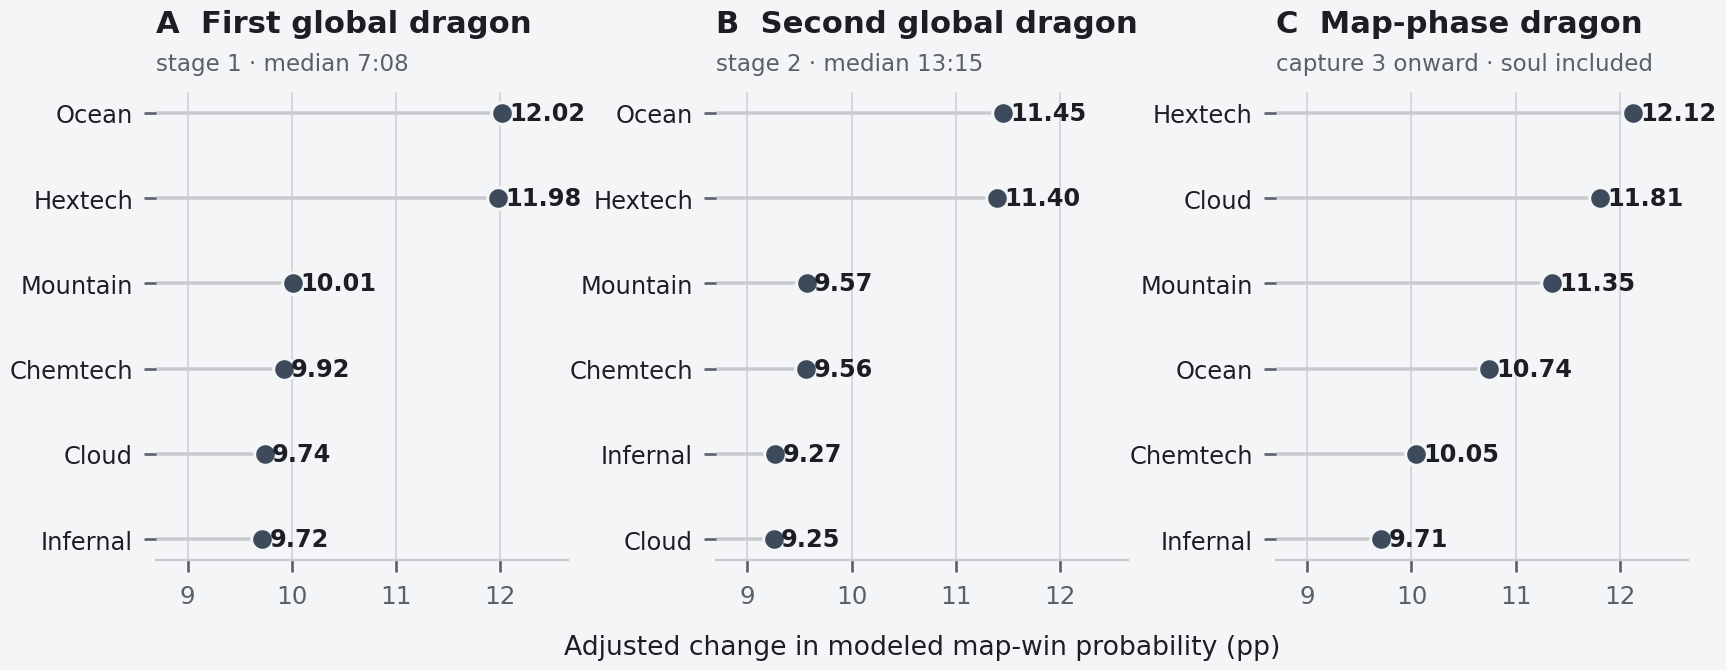
\includegraphics[width=\linewidth]{figures/fig1_stage_rankings.png}
\vspace{-0.25em}
\fineprint{\textbf{Figure 1. Standardized elemental rankings by capture stage.} Each point is a fitted post-minus-pre capture change at the stated reference, averaged over the observed two-team draft mix. The map-phase value averages repeated captures from global capture three through the focal team's fourth stack and soul. Values are associations, not causal buff effects.}
\end{figure}

\begin{center}
\small
\begin{tabular}{@{}lrrrrrr@{}}
\toprule
& \multicolumn{2}{c}{\textbf{First capture}} & \multicolumn{2}{c}{\textbf{Second capture}} & \multicolumn{2}{c}{\textbf{Map phase}} \\
\cmidrule(lr){2-3}\cmidrule(lr){4-5}\cmidrule(lr){6-7}
\textbf{Element} & \textbf{pp} & \textbf{Rank} & \textbf{pp} & \textbf{Rank} & \textbf{pp} & \textbf{Rank} \\
\midrule
Hextech  & +11.98 & 2 & +11.40 & 2 & +12.12 & 1 \\
Cloud    &  +9.74 & 5 &  +9.25 & 6 & +11.81 & 2 \\
Mountain & +10.01 & 3 &  +9.57 & 3 & +11.35 & 3 \\
Ocean    & +12.02 & 1 & +11.45 & 1 & +10.74 & 4 \\
Chemtech &  +9.92 & 4 &  +9.56 & 4 & +10.05 & 5 \\
Infernal &  +9.72 & 6 &  +9.27 & 5 &  +9.71 & 6 \\
\bottomrule
\end{tabular}
\vspace{0.20em}

\fineprint{\textbf{Table 4. Fitted stage matrix.} Ranks order point estimates only. Values are percentage points of modeled map-win probability at the standardized reference.}
\end{center}

\subsection{Why the map-phase ordering changes}
First and second captures are single-stack additions before the map element begins to repeat. The map-phase estimand instead averages a route in which the same element compounds and, on the terminal capture, adds soul. It therefore combines stack coefficients, time interactions, composition interactions, and the fitted soul block. Hextech and Cloud rise in this setting; Ocean falls from first to fourth. Infernal remains last by point estimate in all three columns, but that ranking does not imply that Infernal's mechanical buff is harmful or valueless.

The magnitudes, roughly 9--12 points on average, are larger than a plausible isolated mechanical-buff experiment would ordinarily suggest. The fitted inventory terms can still encode residual objective control, tempo, and map access not removed by the recorded state. The raw capturer won 69.15\% of maps, a selection diagnostic rather than a dragon-value estimate. Standardizing observed associations does not create randomized treatment. The numbers should therefore be read as adjusted model contrasts, not literal causal increments that can be added to a pre-game forecast.

\begin{center}
\small
\begin{tabular}{@{}lrr@{}}
\toprule
\textbf{Observed support} & \textbf{Minimum by element} & \textbf{Maximum by element} \\
\midrule
First captures & 1,037 & 1,121 \\
Second captures & 1,019 & 1,093 \\
Map-phase captures & 2,399 & 2,644 \\
Soul captures & 420 & 489 \\
\bottomrule
\end{tabular}
\vspace{0.20em}

\fineprint{\textbf{Table 5. Capture support behind the standardized matrix.} Counts are observed resolved captures, not the number of synthetic legal contexts scored during standardization.}
\end{center}

\section{Composition-conditioned rankings}
The same element need not have the same fitted marginal value for every draft. Composition enters through pooled own-team and enemy-team trait interactions plus supported champion-element residuals. To make that distinction concrete, Figure 2 fixes both lineups from a Tier 1 LCK example: Gen.G fielded Vayne, Trundle, Cassiopeia, Ziggs, and Shen; T1 fielded Ambessa, Lee Sin, Galio, Jhin, and Camille. All non-inventory state variables are set to the same neutral references used in the overall matrix.

\begin{figure}[h]
\centering
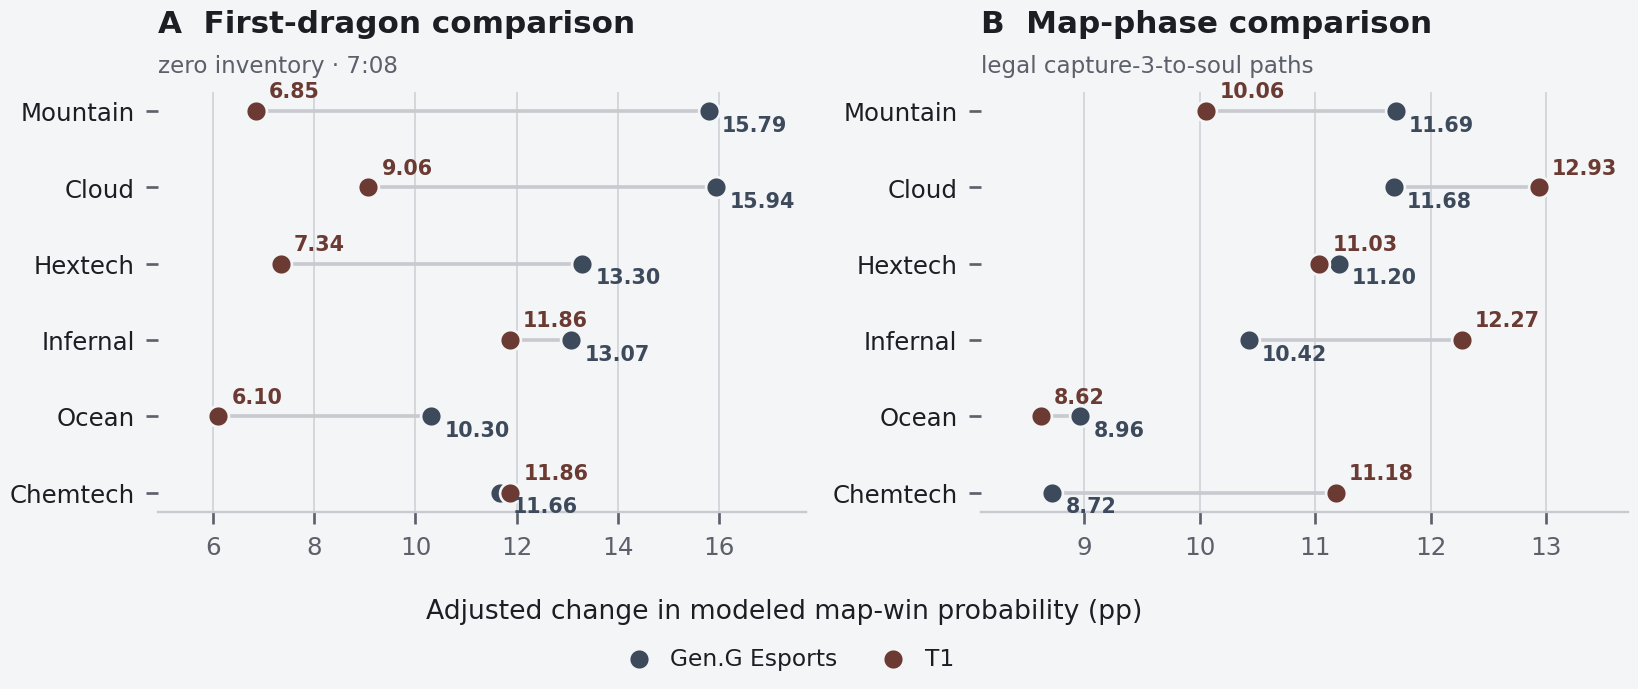
\includegraphics[width=\linewidth]{figures/fig2_composition_example.png}
\vspace{-0.25em}
\fineprint{\textbf{Figure 2. Composition-conditioned marginal associations for one fixed 5v5.} Steel points hold the Gen.G lineup as focal; rust points hold the T1 lineup as focal. Panel A adds the first dragon at 7:08. Panel B averages the legal map-phase routes through soul. The selected champions are evaluated through pooled composition features and supported champion residuals; the figure is not an exact-composition lookup coefficient.}
\end{figure}

For Gen.G, the first-capture point estimates are highest for Cloud (+15.94) and Mountain (+15.79). For T1, Chemtech (+11.86) and Infernal (+11.86) are highest. In the map phase, Gen.G's ordering begins Mountain (+11.69), Cloud (+11.68), and Hextech (+11.20), while T1's begins Cloud (+12.93), Infernal (+12.27), and Chemtech (+11.18). These shifts are large enough to change ordering, but their absolute magnitudes inherit the identification limits of the overall model and have no lineup-specific confidence intervals.

\subsection{What the lineup comparison does and does not use}
The comparison cross-references each champion independently where a supported champion-element cell exists, then adds pooled composition interactions for both teams. It does not search the archive for an exact Gen.G-versus-T1 composition match. The modeled cohort contains 12,214 unique five-champion sides; the median exact side appears once and the maximum appears 57 times. This sparsity is why the model pools composition features instead of fitting exact-lineup cells. It also does not import generic Draft Score synergy or counter coefficients: those estimate a different pre-match association. Exact ally-pair and opponent-pair dragon responses remain zero unless a future family passes its own support and holdout gates.

Role assignment only organizes champion selection in the web interface. It comes from a separate 1,194-map Leaguepedia Cargo draft corpus \cite{leaguepedia}. The GRID model pools champion-element evidence across roles because the compact training compositions lack validated role assignments. Role labels therefore do not change the residual.

\section{Champion-specific evidence}

\subsection{Residual construction}
Every dragon applies to all five champions. The champion layer asks only whether the data support a deviation from the pooled element and archetype association. For champion $k$ and element $e$, the raw residual feature is
\begin{equation}
r_{ke}
=n^{\mathrm{own}}_e\,\mathbf 1(k\in C_{\mathrm{own}})
-n^{\mathrm{opp}}_e\,\mathbf 1(k\in C_{\mathrm{opp}}).
\end{equation}
Eligibility depends on exposure rather than outcome: at least 50 team-games, 25 series, 20 ownership games, 20 non-ownership games, and three organization contexts. Repeated capture rows do not add support. Within each element, the residual vector is constrained to the weighted null space of a pooled intercept and all reviewed archetype tags. Consequently, $\delta_{ke}$ is a ridge-shrunk deviation from the pooled and archetype terms, not a second archetype bonus.

A negative champion residual means ``less positive than the pooled composition expectation'' in the fitted logit. It does not mean the champion loses power from receiving the buff. The common team effect remains present for every champion; individual lines in the web interface allocate deviations around that common effect.

\begin{figure}[h]
\centering
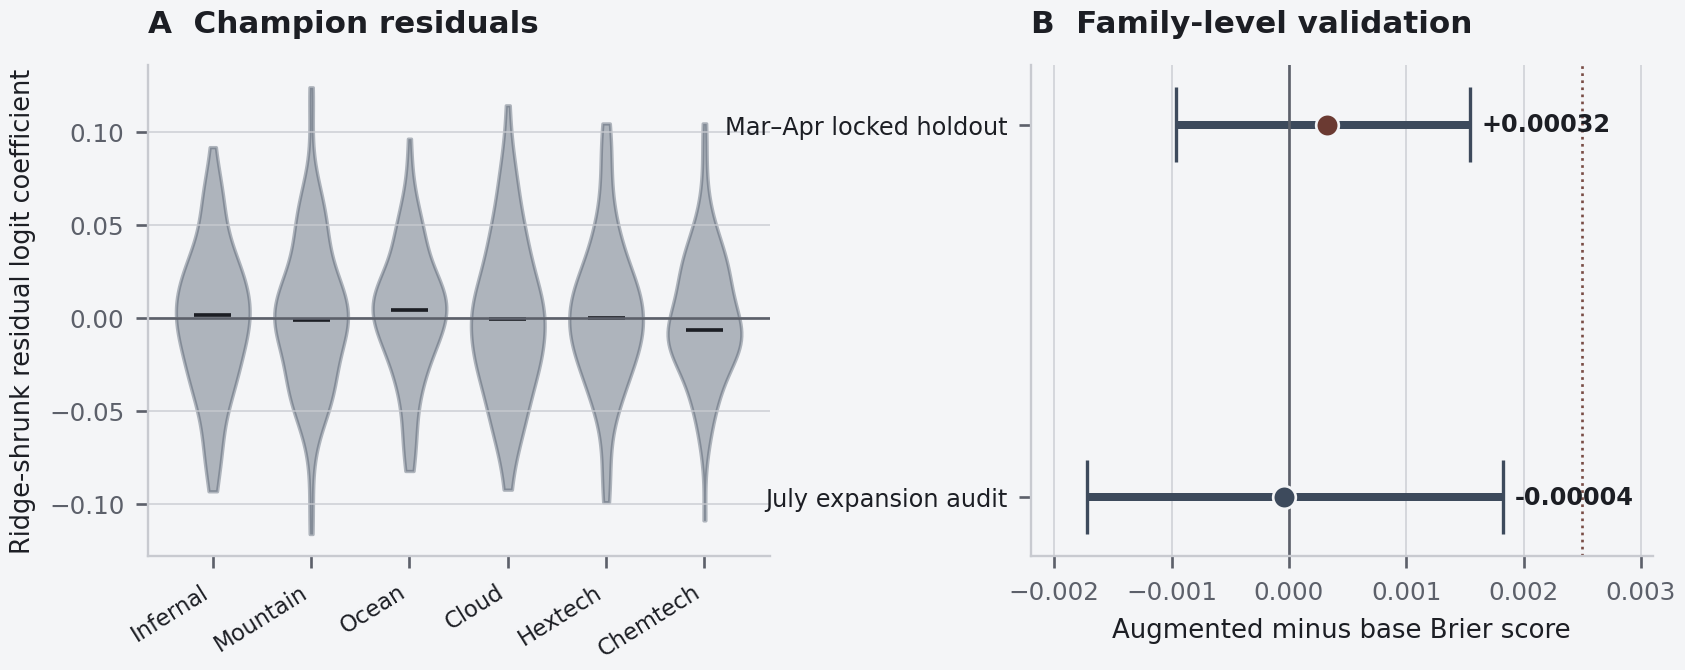
\includegraphics[width=\linewidth]{figures/fig3_residual_validation.png}
\vspace{-0.25em}
\fineprint{\textbf{Figure 3. Champion residual distribution and family-level validation.} Panel A shows the final ridge-shrunk coefficient distributions; they are centered near zero by construction. Panel B reports paired, series-blocked 95\% bootstrap intervals for augmented-minus-base Brier score. Lower is better. The rust dotted line is the prespecified +0.0025 material-regression limit.}
\end{figure}

\subsection{Temporal checks}
The champion layer is exploratory because its use of the March--April window was added after the base holdout protocol had been specified. The initial family uses 331 cells across 59 champions. It improves inner-validation Brier score by 0.00182. On the locked holdout, the augmented model is 0.00032 worse than the frozen base; the series-bootstrap 95\% interval is $[-0.00096,\,0.00154]$, below the material-regression limit.

The publication expansion freezes 547 cells across 93 champions before 1 July and evaluates them on 672 July maps from 327 whole series through 27 July, before the planned 1 August endpoint. Its Brier difference from the frozen base is $-0.00004$, with interval $[-0.00173,\,0.00182]$. After this family-level gate passes, the final full-cohort refit contains 549 cells. Two cells first clear the exposure rule only in the final refit and carry no cell-level holdout claim.

\begin{center}
\begin{minipage}{\linewidth}
\centering
\small
\begin{tabular}{@{}lrrrrrrr@{}}
\toprule
\textbf{Vocabulary} & \textbf{Champions} & \textbf{Cells} & \textbf{Inf.} & \textbf{Mtn.} & \textbf{Ocn.} & \textbf{Cld.} & \textbf{Hex./Chem.} \\
\midrule
March--April evaluation & 59 & 331 & 55 & 52 & 58 & 57 & 54 / 55 \\
Pre-July audit & 93 & 547 & 91 & 90 & 92 & 90 & 92 / 92 \\
Final publication & 93 & 549 & 91 & 91 & 92 & 90 & 92 / 93 \\
\bottomrule
\end{tabular}
\vspace{0.20em}

\fineprint{\textbf{Table 6. Champion-element vocabulary.} Temporal checks validate the residual family and vocabulary-expansion procedure. They do not validate every coefficient independently.}
\end{minipage}
\end{center}

\section{Threats to validity and reproducibility}

\subsection{Identification and transport}
\begin{itemize}
\item \textbf{Capture is selected.} The data do not randomize which team receives a dragon. Recorded state controls reduce but cannot remove unmeasured priority, vision, position, cooldowns, or strategic access.
\item \textbf{No take-versus-leave policy is identified.} The alternative action and cross-map compensation are not observed as a complete decision node. The resolved-allocation layer therefore remains diagnostic.
\item \textbf{Ranks lack effect uncertainty.} The artifact provides predictive holdout metrics and champion-family bootstrap gates, but no confidence interval or rank probability for the standardized stage effects.
\item \textbf{Composition terms are pooled.} Exact 5v5, stage-specific champion, champion-soul, ally-pair, and enemy-pair effects are disabled. The fixed-lineup example is a model evaluation, not empirical support for that exact composition.
\item \textbf{Professional circuits are pooled.} Tier 1, international, and other pro games contribute to one model with competition controls. No subgroup independently reaches the requested 6,000-map normalization.
\item \textbf{Patch and provider drift remain possible.} Exact patch coverage is audited, but the fitted association spans a changing professional environment. Provider-side corrections after the snapshot would require a new content-addressed artifact.
\item \textbf{State and taxonomy are imperfect.} Capture state may lag by as much as 60 seconds; complete-composition, reviewed-archetype, and complete-roster coverage are 98.23\%, 96.67\%, and 97.32\%. Champion archetypes are static reviewed labels rather than learned kit simulations.
\end{itemize}

\subsection{Data minimization and lineage}
GRID source archives and credentials are not distributed. While streaming the provider data, the pipeline projects only the columns needed for game identity, draft, capture path, and pre-capture state. The normalized inputs are content-addressed:

\begin{center}
\scriptsize
\begin{tabularx}{\linewidth}{@{}lYl@{}}
\toprule
\textbf{Artifact} & \textbf{SHA-256} & \textbf{Bytes} \\
\midrule
\texttt{games.parquet} &
\texttt{ef7a5eaf7d2f15726a8d889be5e4a1c06b90ed924267e667161d37c241df4382} &
508,130 \\
\texttt{events.parquet} &
\texttt{d0dd3b1b5d42bdc1e8c43c8317270db9bbfd40ac510ae134cb87c01583898ad9} &
1,450,994 \\
\texttt{draft\_archetypes.py} &
\texttt{e5927d55d736df4e1c129b30b4a7aab6b7ab8ccade02d91725088038c7f09a18} &
10,932 \\
\shortstack[l]{\texttt{elemental\_drake\_explorer\_}\\\texttt{model.json}} &
\texttt{12a55d208f41afdeb4428e691824a8e069b76d4db12402889da214f6bfd1687d} &
3,440,186 \\
\bottomrule
\end{tabularx}
\end{center}

The public web application contains only the derived runtime, support metadata, aggregate coverage, champion taxonomy, and seven curated examples. Stable provider identifiers are omitted. A four-series raw reconciliation audit compared 21 capture events and matched element, owner, and time within two seconds for all 21.

\section{Discussion}
\subsection{There is no stage-free winner}
At the population average, the simplest summary is stage-specific. Ocean and Hextech are effectively tied at the first two captures by fitted point estimate. Hextech, Cloud, and Mountain lead the repeated map phase. The change in ordering is not a contradiction: the estimands condition on different legal pre-inventories and only the map-phase quantity includes the route to soul.

\subsection{Composition matters, but precision matters too}
The fixed 5v5 example confirms that the model can reorder elements when both drafts change. That is the intended use of arbitrary champion selection in the web application. It should not be presented as ``this exact composition has historical proof'' or as a deterministic recommendation. The defensible description is: the model combines pooled team traits with regularized champion-element evidence, then evaluates the selected lineups at a fixed state.

\subsection{What would be needed for decisions}
Operational advice requires a model of the choice to start, contest, trade, or leave the objective. A future study would timestamp the decision before commitment and record positions, health, cooldowns, summoners, vision, lane states, cross-map farm, and plausible opponent responses. With those inputs, one could compare
\begin{equation}
\mathbb E\!\left[
Y_i(\text{take or contest})-Y_i(\text{leave or trade})
\mid\mathcal I_{\mathrm{pre}}
\right],
\end{equation}
with team- and patch-grouped evaluation. The present inventory model is useful context for that decision model, but it is not a substitute for it.

\section{Conclusion}
Three conclusions survive a conservative reading of the current artifact:
\begin{itemize}[leftmargin=1.2em,itemsep=0.28em,topsep=0.20em]
\item \textbf{First and second dragon: Ocean and Hextech are the leading pair.} Ocean ranks first at +12.02 and +11.45 points, but its fitted gaps over Hextech are only 0.04 and 0.05 points. The paper does not claim those gaps are statistically resolved.
\item \textbf{Map phase: Hextech leads, with Cloud close behind.} Their fitted averages are +12.12 and +11.81 points when legal routes from global capture three through soul are weighted equally.
\item \textbf{Composition can change the ordering.} Pooled draft interactions and 549 regularized champion-element cells support fixed-lineup exploration, subject to family-level rather than cell-level validation.
\end{itemize}

The values are best read as a structured map of adjusted professional-game associations. They make the stage and lineup assumptions explicit, while leaving the causal question---whether a team should take, contest, trade, or leave a particular dragon---open.

\begin{thebibliography}{99}
\scriptsize
\setlength{\parskip}{0pt}
\setlength{\itemsep}{0pt}
\setlength{\parsep}{0pt}
\bibitem{grid} GRID. \href{https://grid.gg/get-league-of-legends/}{\textit{League of Legends data through the GRID Open Platform}}. Accessed 28 July 2026.
\bibitem{riot1320} Riot Games. \href{https://www.leagueoflegends.com/en-sg/news/game-updates/patch-13-20-notes/}{\textit{Patch 13.20 Notes}}. 2023.
\bibitem{riot136} Riot Games. \href{https://www.leagueoflegends.com/en-au/news/game-updates/patch-13-6-notes/}{\textit{Patch 13.6 Notes}}. 2023.
\bibitem{riot1222} Riot Games. \href{https://www.leagueoflegends.com/en-us/news/game-updates/patch-12-22-notes/}{\textit{Patch 12.22 Notes}}. 2022.
\bibitem{leaguepedia} Leaguepedia. \textit{Cargo ScoreboardPlayers and ScoreboardGames tables}. Accessed 28 July 2026.
\bibitem{scryglass} Scryglass. \href{https://scryglass-elemental-drakes.vercel.app}{\textit{Elemental Drakes interactive study}}. Model artifact generated 28 July 2026.
\end{thebibliography}

\end{document}
